% THIS IS SIGPROC-SP.TEX - VERSION 3.1
% WORKS WITH V3.2SP OF ACM_PROC_ARTICLE-SP.CLS
% APRIL 2009
%
% It is an example file showing how to use the 'acm_proc_article-sp.cls' V3.2SP
% LaTeX2e document class file for Conference Proceedings submissions.
% ----------------------------------------------------------------------------------------------------------------
% This .tex file (and associated .cls V3.2SP) *DOES NOT* produce:
%       1) The Permission Statement
%       2) The Conference (location) Info information
%       3) The Copyright Line with ACM data
%       4) Page numbering
% ---------------------------------------------------------------------------------------------------------------
% It is an example which *does* use the .bib file (from which the .bbl file
% is produced).
% REMEMBER HOWEVER: After having produced the .bbl file,
% and prior to final submission,
% you need to 'insert'  your .bbl file into your source .tex file so as to provide
% ONE 'self-contained' source file.
%
% Questions regarding SIGS should be sent to
% Adrienne Griscti ---> griscti@acm.org
%
% Questions/suggestions regarding the guidelines, .tex and .cls files, etc. to
% Gerald Murray ---> murray@hq.acm.org
%
% For tracking purposes - this is V3.1SP - APRIL 2009

\documentclass{acm_proc_article-sp}
\usepackage[numbers, sort, compress]{natbib}
\usepackage{graphics}
\usepackage{graphicx}
\usepackage{epstopdf}
\usepackage{color}
\usepackage{hyperref}
\usepackage{pdfsync}
\usepackage{mdwlist}

\begin{document}

%\title{A Sample {\ttlit ACM} SIG Proceedings Paper in LaTeX
%Format\titlenote{(Does NOT produce the permission block, copyright information nor page numbering). For use with ACM\_PROC\_ARTICLE-SP.CLS. Supported by ACM.}}

\newif\ifdraft
\drafttrue                                                                                                   

\ifdraft
 \newcommand{\rananote}[1]{ {\textcolor{blue}    { ***Omer:     #1 }}}
 \newcommand{\jkimnote}[1]{{\textcolor{green}   { ***Joohyun:   #1 }}}
 \newcommand{\jhanote}[1]{  {\textcolor{red}     { ***SJ: #1 }}}
  \newcommand{\smnote}[1]{  {\textcolor{blue}     { ***sharath: #1 }}}
 \newcommand{\todo}[1]{  {\textcolor{red}     { ***TODO: #1 }}}
 \newcommand{\fix}[1]{  {\textcolor{red}     { ***FIX: #1 }}}

\else
 \newcommand{\rananote}[1]{}
 \newcommand{\jkimnote}[1]{}
 \newcommand{\jhanote}[1]{}
 \newcommand{\todo}[1]{  {\textcolor{red}     { ***TODO: #1 }}}
 \newcommand{\fix}[1]{}                                                                                     
\fi

\title{Characterizing Deep Sequencing Analytics Using BFAST: Towards a
  Scalable Distributed Architecture for Next-Generation Sequencing
  Data}

% \title{Exploring the RNA Folding Energy Landscape with
%   Boltzmann-Weighted Sampling of Secondary Structures: Enhancing the
%   Biological Discovery with Adaptive Distributed Application
%   Management System (ADAMS) }

%\subtitle{[Extended Abstract]
%\titlenote{A full version of this paper is available as
%\textit{Author's Guide to Preparing ACM SIG Proceedings Using
%\LaTeX$2_\epsilon$\ and BibTeX} at
%\texttt{www.acm.org/eaddress.htm}}}
%
% You need the command \numberofauthors to handle the 'placement
% and alignment' of the authors beneath the title.
%
% For aesthetic reasons, we recommend 'three authors at a time'
% i.e. three 'name/affiliation blocks' be placed beneath the title.
%
% NOTE: You are NOT restricted in how many 'rows' of
% "name/affiliations" may appear. We just ask that you restrict
% the number of 'columns' to three.
%
% Because of the available 'opening page real-estate'
% we ask you to refrain from putting more than six authors
% (two rows with three columns) beneath the article title.
% More than six makes the first-page appear very cluttered indeed.
%
% Use the \alignauthor commands to handle the names
% and affiliations for an 'aesthetic maximum' of six authors.
% Add names, affiliations, addresses for
% the seventh etc. author(s) as the argument for the
% \additionalauthors command.
% These 'additional authors' will be output/set for you
% without further effort on your part as the last section in
% the body of your article BEFORE References or any Appendices.

\numberofauthors{6} %  in this sample file, there are a *total*
% of EIGHT authors. SIX appear on the 'first-page' (for formatting
% reasons) and the remaining two appear in the \additionalauthors section.
%
\author{
% You can go ahead and credit any number of authors here,
% e.g. one 'row of three' or two rows (consisting of one row of three
% and a second row of one, two or three).
%
% The command \alignauthor (no curly braces needed) should
% precede each author name, affiliation/snail-mail address and
% e-mail address. Additionally, tag each line of
% affiliation/address with \affaddr, and tag the
% e-mail address with \email.
%
\alignauthor Joohyun Kim\\
       \affaddr{Center for Computation and Technology}\\
       \affaddr{Louisiana State University}\\
       \affaddr{216 Johnston}\\
       \affaddr{Baton Rouge, LA} \\
       \email{jhkim@cct.lsu.edu}
\alignauthor Sharath Maddineni\\
       \affaddr{Center for Computation and Technology}\\
       \affaddr{Louisiana State University}\\
       \affaddr{216 Johnston}\\
       \affaddr{Baton Rouge, LA}
\alignauthor Shantenu Jha\titlenote{Author for correspondence}\\
      \affaddr{Center for Computation and Technology}\\
     \affaddr{Louisiana State Unvierstiy}\\
      \affaddr{214 Johnston}\\
      \affaddr{Baton Rouge, LA}
     \email{sjha@cct.lsu.edu}
}
% There's nothing stopping you putting the seventh, eighth, etc.
% author on the opening page (as the 'third row') but we ask,
% for aesthetic reasons that you place these 'additional authors'
% in the \additional authors block, viz.
%\additionalauthors{Additional authors: John Smith (The Th{\o}rv{\"a}ld Group,
%email: {\texttt{jsmith@affiliation.org}}) and Julius P.~Kumquat
%(The Kumquat Consortium, email: {\texttt{jpkumquat@consortium.net}}).}
\date{28 Feb. 2010}
% Just remember to make sure that the TOTAL number of authors
% is the number that will appear on the first page PLUS the
% number that will appear in the \additionalauthors section.

\maketitle
\begin{abstract} 

  Next-Generation (gene) Sequencing (NGS) platforms produce
  significantly larger amounts of data compared to early Sanger technology sequencers.
  In addition to the challenges of data-management that arise from
  unprecedented volumes of data, there exists the important
  requirement of effectively analyzing the data.  In this paper, we
  use BFAST -- genome-wide mapping application, as a representative
  example of the typical analysis that is required on data from NGS
  machines.  We investigate two model genomes -- human genome and a
  microbes -- {\it Burkerholderia Glumae}, that represent an
  eukaryotic and a prokaryotic system.  The computational complexity
  of genome-wide mapping using BFAST, depends upon the size of a
  reference genome, the data size of short reads, amongst other
  factors.  We analyze the performance characteristics of BFAST and
  understand its dependency on different input
  parameters. Characterizing the performance suggests that genome-wide
  mapping benefits from both scaling-up and scaling-out; in fact, for
  certain problem instances, scaling-out is a critical requirement for
  performance.  We then design, develop and demonstrate a
  runtime-environment that supports both the scale-up and scale-out of
  BFAST over production grid and cloud environments.
  
  % from high-throughput technologies of the Next Generation
  % Sequencing platforms and their biological genome contexts such as
  % distinctive differences between prokaryotes vs eukaryotes.
  
%   We then investigate the use of distributed computing environments, a
%   production HPC grid and a cloud environment for the genome-wide
%   mapping with BFAST.  The two distributed environments, the Louisiana
%   Optical Network Initiative (LONI) grid and a Cloud system from the
%   FutureGrid, were used primarily focusing on different and unique
%   challenges in HPC and Cloud computing conditions.

\end{abstract}

\category{D.1.3}{Software}{Concurrent Programming}{distributed programming/parallel programming}
\category{J.3}{Computer Applications}{Bioinformatics, Mapping}


% A category with the (minimum) three required fields
%\category{H.4}{Information Systems Applications}{Miscellaneous} %Acategory including the fourth, optional field follows...
%\category{D.2.8}{Software Engineering}{Metrics}[complexity measures,performance measures]

\terms{Theory, Cyberinfrastructure, Analysis} \keywords{Genome Sequence Alignment, BFAST, Human Genome, Burkerholderia Glumae
  Runtime Environment, Distributed Computing, Simple API for Grid
  Applications (SAGA), Pilot-Job abstraction}

%\keywords{ACM proceedings, \LaTeX, text tagging} % NOT required for Proceedings 
\keywords{RNA conformation energy landscape, Runtime Environment, SAM-I riboswitch,
 S gene of Bovine Corona Viral Genome} % NOT required for Proceedings

\section{INTRODUCTION} 

High-throughput genome sequencing techniques provided by Next
Generation Sequencing (NGS) platforms are changing biological sciences
and biomedical research dramatically.  These techniques have led to a
broadening of sequencing capabilties and access to comprehensive
genome-wide information at increasingly lower costs compared to
previous sequencing techniques (such as those based on Sanger
sequencing)
\cite{metzker2010,mardis2008-tig,mardis2008-arghg,gilad2009,mortazavi2008,sorek2010}.
Thanks to advances in deep sequencing protocols such as ChIP-seq and
RNA-seq, high-throughput sequencing techniques have become essential
methodologies in studies of cell development and
differentiation\cite{wang2009-natrevgen,pepke2009,gilad2009,mortazavi2008,sorek2010}.
The resulting influx of biological information about the genome-wide
organization and the interaction map of target genes and pathways that
reveal underlying mechanisms of gene expression and regulation in a
living cell. This has the potential to lead to discoveries of remedies
for various diseases such as cancer, infectious diseases, and
dysfunctional diseases caused genetically or by
aging\cite{amaral2008,encode2007,baek2008,costa2009}.


While high-throughput techniques enjoy extremely high coverage of
target genome regions, as referred to by the term, "deep sequencing",
the current technologies adopted by NGS platforms such as Illumina GA
II and Applied Biosystems SOLiD are limited to generating only short
sequence reads, generally less than 100 hundred
nucleotides\cite{metzker2010}.  

Consequently, it has become a computational challenge to map these
high volume short reads onto a reference genome or de novo assembly
that are needed as the first step for any genome-wide
studies\cite{alex2009,trapnell2009,scheibye-alsing2009,pop2002,hernandez2008,farrer2008}.
It is expected that data-sets of interest will increase by several
orders of magnitude as the number of genomes that need to be sequenced
together increases exponentially.  This is a result of comparative
genomics as well as genome-wide variation studies that require a
statistical number of genomes for one single species as shown in the
recent 1000 genome project and human genome
studies\cite{1000genome,mardis2008-tig,gilad2009,alex2009,kim2011}.

%challenge immediately mapping process on to a reference genome or 
% Consequently, these high volume short reads challenge immediately
% mapping process on to a reference genome or de novo assembly that are
% needed as the first step for any genome-wide
% studies\cite{alex2009,trapnell2009,scheibye-alsing2009,pop2002,hernandez2008,farrer2008}.

To address these challenges, there have been algorithmic advances and
several tools implementing these advances are becoming available
\cite{trapnell2009,bfast2009,scheibye-alsing2009,pepke2009,samtools}.
Whereas such algorithmic advances and introduction of new tools have
been consistently led by the computational biology community, the
development of a well-architected integrated infrastructure -- the
software \& services, data management capabilities and user interfaces
has received less attention.  As we will demonstrate, NGS analysis is
not a simple compute or data-intensive application, but an interesting
mix of high-end and high-throughput computing with data-intensive
requirements.  We ask the fundamental question: what is the
appropriate architecture of the infrastructure to address the existing
computational requirements of NGS analysis, data-set volumes -- now
and extrapolating into the future?  The need for an appropriate
scalable and flexible architecture for the infrastructure, becomes
prelevant because the computational complexity of the specific problem
instance is often influenced by the biological characteristics of the
target genome(s), the volume of relevant genomics data.

%\jhanote{not sure what to do with the following paragraph} One
%important caveat is that as advances of genome sequencing technologies
%evolve further in the future with innovations, for example, such as a
%single molecule sequencing technology and ever-growing genome data,
%any computational algorithms or implementations with a bioinformatic
%tool are subject to change to respond such progresses or will become
%less useful if the tool do not meet new conditions.

Our approach is to primarily focus on the mapping process of short
reads from NGS platforms against a reference genome.  The mapping is
carried out with the tool, BFAST\cite{bfast2009, bfast2009b} which was
chosen specifically considering its capability to support parallel and
multi-threading execution.  Our investigation with this bioinformatic
program would represent a general situation for a bioinformatics tool
employed for genome-wide analysis infrastructure.  As a use case, we
understand the computational complexity of BFAST\cite{bfast2009,
  bfast2009b} and the determinants of its performance for two
exemplary genomes, human genome and a microbial genome {\it
  Bukerholderia Glumae}.
 
Having understood the computational requirements, and the importance
of both scaling-up and scaling-out, we present our initial design
objectives and a prototype infrastructure that seamlessly uses
High-Performance Computing (HPC) grids and Cloud environment for
genome-wide analysis.  Our infrastructure builds upon existing
capabilities of the Distributed Adaptive Runtime Environment (DARE)
framework -- with enables the seamless utilization of heterogeneous
distributed computing resources.  DARE provides an existing efficient
framework upon which to build a scalable infrastructure to support a
wide range of abstractions and execution requirements for the
analytics required for NGS data.

This paper is organized as follows....

% are keenly utilized for a scalable computation of a target genome-wide
% analysis tool.


% patterns while recognizing the potential scalability of
% deployable computing resources.
% abstraction and 

% characteristics of biological information in conjunction with the
% capability of the target scientific application, and then, to analyze
% computational complexity for carrying out mapping process with two
% exemplary genomes, human genome and a microbial genome, Bukerholderia
% Glumae.  Base on the results with this analysis, we present the use of
% the runtime environment developed with the Distributed Adaptive
% Runtime Environment (DARE) framework, which is built upon SAGA/BigJob
% abstraction and provides an efficient framework for building
% biological information infrastructure supporting a wide range of
% execution patterns while recognizing the potential scalability of
% deployable computing resources.
% Our development with a federated HPC
% grid, Louisiana Optical Network Initiative (LONI) and a Cloud
% environment in the FutureGrid is desribed largely focusing on the
% comparative analysis on execution of mapping process in each
% environment.

\section{Mapping Genomes: Characterizing BFAST and Understanding
  the Challenges}

\subsection{BFAST: Application}

\jhanote{Need to be consistent with usage of ``problem instance'',
  ``application'' and ``tool''. I propose the human genome/glumae are
  the problem instances, Bfast is the application and the BigJob etc
  are execution tools}

The application used to target genome analysis is
BFAST\cite{bfast2009,bfast2009b}, which is used for genome-wide
mapping.  In brief, BFAST requires a reference genome sequence and NGS
platform generated short reads initially and produces mapping results
of billions of short reads onto a target reference genome.  Notable
key common features include: i) a requirement of input data containing
sequence information of a reference genome or short reads from NGS
platforms ii) a production of output information that is generally
written with a format that is successively injected to another tool as
input.


% which is also critically considered with the development of
% BFAST\cite{bfast2009}.  represents a class of tools that comprises
% diverse genome-wide analysis applications but shares similar
% computational features.  The parallel strategy suggested by BFAST
% lies primarily in the

% \jhanote{What does ``d'' in the bfast manual stand for? Please use the
%   same notation.. as opposed to introducing new notation such as ``low
%   memory''}

BFAST employs a pipeline approach, and in fact as summarized in
Fig.~\ref{fig:workflow-bfast} and Table~\ref{table:bfast-summary},
BFAST mapping is carried out as a pipeline that comprises six
different steps. Of these three steps (creation of an index of a
ref. genome, finding CALs, and alignment of CALs), can be executed in
parallel or multi-threading support options.
 
In order to facilitate the utilization of the (single) resource that
is employed, the index file can be suitably created, and the possible
fragmentation of data sets. For example, short reads can be stored in
multiple files and mapping of short read in each file can be conducted
independently.
 
There can be large variation in the data volume -- input, output,
and/or temporary files, often requiring that BFAST should support
different (local) execution modes.  BFAST supports classic space-time
tradeoff capabilities, i.e., memory and disc usage versus
time-to-solution taken. BFAST can be run using multi-threads (ideally
on a multi-core machine).

Specifically, BFAST supports multi-threading and a ``low memory''
option for "bfast match" step, which finds CALs of each short read in
indexes of a reference genome.  The low option aims specifically to
split the index files into several files, and thereby facilitating low
(peak) memory consumption.  The number of threads is determined by the
parameter (\texttt{-n}); the \texttt{-d} option is used to split the
index into multiple parts in order to support low-memory computation

%of indexed into many files, requiring a lower memory.  
%where d is the parameter for the low memory
                 %consumption 
%is suitable for a large range of architectures;

Note that unlike short reads, the whole reference genome is required;
thus the \texttt{-d} option is useful for specific architectures (with
low memory); but as we present later, it requires more computing time
due to multiple indexing for a given read.  The number of index files
generated with the \texttt{-d} flag is $N_i$, which equals $n_m \times
4^d$, where $4^d$ files are generated by splitting one index file and
$n_m$ is the number of masks for indexing, and usually fixed as 10 for
our work.  For example, $d=0$ creates 10 index files, whereas $d=1$
creates 40 index files ie four index files are generated for each mask
and processed sequentially.  

Additionally, BFAST supports multi-threading as an input option for
the three computationally demanding steps.  Taken together, BFAST can
support varying degrees and types of parallelism or multi-threading,
and thus suitable for modern processor architectures.  In particular,
appreciating the possible data fragmentation that is in many cases the
consequence of biological nature of genome data and produced from
genome information.

\begin{figure}
 \centering
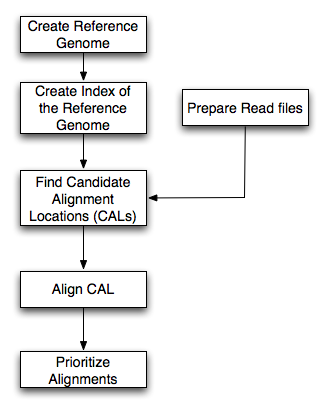
\includegraphics[scale=0.45]{figures/workflow.png} 

\caption{\small Overall workflow for a mapping procedure using BFAST.
  In this work, we focus on the step for finding Candidate Alignment
  Locations (CALs).}
  \label{fig:workflow-bfast} 
\end{figure}

\begin{table}
\small
\begin{tabular}{|c|c|c|c|} 
  \hline BFAST & Description & Features for \\ command & & Parallelism
  \\ \hline \hline \texttt{bfast fasta2brg} & creation of & multiple \\ &a ref. genome &
  independent \\ & & contigs \\ \hline
  \texttt{bfast solid2fastq} & preparation of & multiple sequence \\ & short
  read files & read files\\ \hline

\texttt{bfast index} & creation  & multi-threading \& \\
& of reference  & low memory  \\ 
&genome indexes&option \\
 
  \hline
\texttt{bfast match} & finding Candidate   &  multi-threading \& \\

& Alignment &  parallel execution \\
& Locations (CALs) & \\\hline
\texttt{bfast localalign} & alignment of&   parallel execution \\
&  each CAL   & \\

  \hline
\texttt{bfast postprocess} & prioritization   &  parallel execution \\ 
& of alignments & \\
\hline


\hline
\end{tabular} \caption{Description of BFAST commands and features for parallel and multi-threading execution}
 \label{table:bfast-summary} 
\end{table}

In spite of the fact that BFAST has by design been made suitable to
exploit the computing capabilities of a range of modern processor
architectures, it is valid to ask if there remains other bottlenecks
(eg data flow/access) in the utilization of such architectures?
Additionally, if the answer if found to be positive, it is natural to
ask whether appropriate runtime environments can be developed in order
to overcome these limitations, and to enable BFAST's effective use of
distributed architectures?

\subsection{BFAST: Characteristics}


\begin{figure}
 \centering
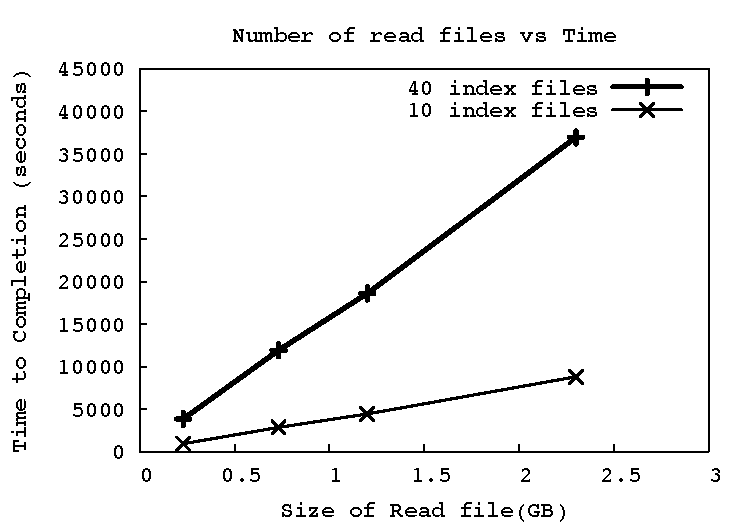
\includegraphics[scale=0.66]{figures/readsvstime.pdf}
%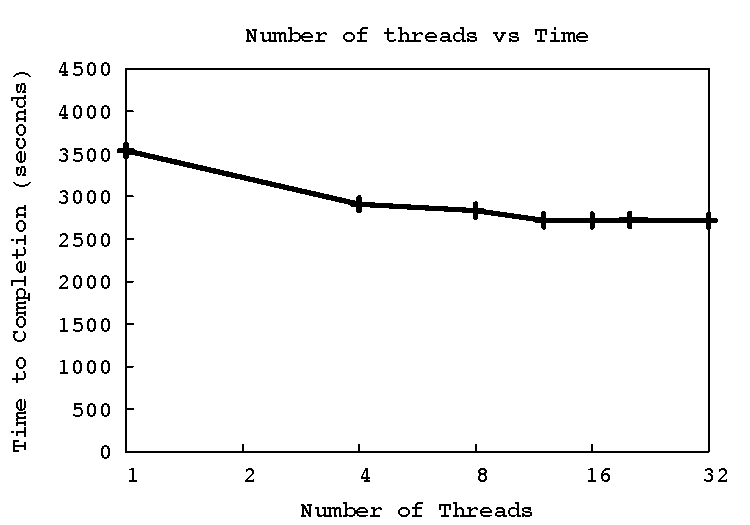
\includegraphics[scale=0.66]{figures/threadsvstime.pdf} 

\caption{\small The time-to-completion of the 'bfast match' step is
  measured by varying the size of short read file.  Two lines
  represent two cases differing in the low memory option, which
  results in the different number of index files.  Human genome (hg18)
  chromosome 21 is used as the reference genome. }
  \label{fig:parallel-execution} 
 \end{figure}


\begin{table}
\begin{tabular}{|c|c|c|c|} 
  \hline 
   & Human (hg18) & Burkerholderia   \\ 
& & Glumae (BGR1)\\   
   
   \hline
 \underline{Reference Genome} & &  \\
    \# of base pairs (bp) &  3 Gbp & 7.3 Mbp \\
   Genome Structure &   23 chromosome  & 2 chromosomes  \\  
   &   pairs & \& 4 plasmids \\
    Volume of indexes  & approx. 12 GB  & approx. 447 MB  \\
      \hline
    \underline{Short Reads} & &   \\
        \underline{Sequence Data}& &    \\
  Type of  &  Exome  & Whole \\
  
Genome Analysis  &  &  Genome \\
&& Resequencing \\
  Sequencing Platform & ABI SOLiD  &  Illumina GA2 \\
  Sequencing   & 8.7 GB & 5.4 GB \\
  Data Volume&&\\
  
  
  \hline
  \underline{BFAST indexing} & &  \\
  Minimal disk &  approx. 130 GB   &    approx. 0.437 GB   \\
space required & &\\
\hline
\end{tabular} \caption{The information about the size of reference genomes, volumes of datasets from
 Next Generation Sequencing (NGS) platforms and disk space required during the mapping calculation 
 with BFAST is summarized assuming all calculations are carried out with a single machine.}
 \label{table:two-genomes} 
\end{table}
First, performance gains with multi-threading are marginal showing only 30 \% speed up when reaches the 
limit with all of the number of free cores being used.  Also, it is apparent that the option has a limitation only
until the number of required thread becomes equal to the total available cores in a given system, 
12 cores in the case of results in Fig.~\ref{fig:parallel-execution}.

\subsubsection{Computational Requirements}

An understanding of computational requirements for carrying out BFAST steps, in particular the "bfast match" step,is 
critically important for a infrastructure development in which a target genome-wide analysis tool is effectively provided 
to a scientific community as a scalable application, the overall execution of BFAST, or any short read mapping tool, 
is dependent upon biological contexts such as a type of a target reference genome and a high-throughput sequencing 
technique generating short read sequences, data structure for parallel/concurrent execution, parallelism support such
 as multi-threading, and more importantly the utilization of such parameters with available computing architectures with 
 respect to parallel execution capabilities and data management.  

In Table~\ref{table:two-genomes}, we summarize the information related to such parameters. 
For example, we investigated two genome datasets that are representative of biological diversity, 
an eucaryote system, human, and a microbe, Burkerholderia Glumae\cite{kim2011}.  Two genomes 
differ in the size and the genome structure of reference genomes, and types of sequencing protocols.  
Importantly, the two different genomes display widely different data sizes in terms of the reference
genome sequence, short reads data, and required disk space for carrying out the mapping with BFAST. 

As an investigation for computational requirements, first, we measure the time-to-completion for "bfast match"
 step while varying the size of a read file.  The results as shown in Fig.~\ref{fig:parallel-execution}, it is found
  that a linear scaling in time-to-completion vs. the size of read file is well satisfied, indicating the parallel option 
  with multiple read files is a useful strategy of scaling out, i.e.  using more cores with a smaller size of read files.  
  Secondly, the low memory option that creates more index files require a longer calculation time as found 
  with the comparison between 40 index files $(d = 1)$ vs. 10 index files ($ d = 0 $) ($n_m = 10$ is used).   


% \jhanote{Joohyun: Please organize each description addressing each of
%   the following points: (i) Brief outline of the scientific problem,
%   (ii) What are the challenges, (iii) estimates of volumes of data
%   involved, distributed or not?, number of tasks, are they coupled or
%   uncoupled -- what is the level of coupling between tasks?}



% \begin{table}
 %\begin{tabular}{|c|cc|} 
 %\hline 
%Distributed &  HPC Grid &  Cloud \\ 
%Environment && (Eucalyptus)\\
%\hline
% &  Louisiana Optical & FutureGrid \\
%& Network Initiative  & \\
%System  Name &  QB/Small Linux Clusters   &  INDIA/SIERRA \\
%Disk Space  Limit  &  QB : unlimited  &    \\
%                         &  Small Linux Clusters : 100 GB  &  \\
 %\hline
 %\end{tabular}
%\caption{Specification of two distributed environments.  \jkimnote{need to fill Cloud systems}}
%\label{table:two-systems} 
%\end{table}
 
\subsubsection{Characterising Data Requirements}

The Table~\ref{table:dynamic-diskspace} dynamic diskspace required
during the runtime of bfast match step.  The disk space required for
each read file is constant with given sizes. The bfast match creates
several temporary files during runtime. A rough estimate of these
temporary files include a temporary file for read file, a temporary
file for each index mask and there are 10 index masks used in this
case so ten temporary, some more temporary files depending on the d
option while preparing indexes ($d=0$: 1 temporary file, $d=1$: 4
temporary files).  However, all these temp files are emptied once
"bfast matching step" completes.  It can be estimated that there will
be around 16 temporary files in case A for to process each each read
files. The size of each temporary file observed was 105MB. Thus for
each read to process it requires around 1.68 GB. If all the bfast
matches processed concurrently the we require 40 times the diskspace
required for each matching(40$\times$1.68).  The diskspace for other cases
can also calculated similarly. The disk space was calculated with
respect to this particular configuration and may vary unpredictably
with other configurations.

\begin{table}
 \begin{tabular}{|c|c|c|c|c|c|} 
 \hline 
Case &Read& Index& Size &  Num. of & Approx.  \\
 &files &  files  & Temp file & Temp files & disc space\\
 \hline
A&40 & 40 &105MB & 16 &67 GB \\
B&20 & 40 & 220MB & 16 &70 GB \\
C&40 & 10 & 105MB & 13 &52 Gb \\ 
 \hline
 \end{tabular}
 \label{table:dynamic-diskspace} 
 \caption{This table shows the required disk space when all the read files
   are processed concurrently with different number of read files and
   index files. The Reference genome used is Human Genome 18
   Chromosome 21 and total size of read files was 8.9 GB.}
\end{table}

The disk space required in concurrent run of several read files in
matching phase is important because if the amount of disk space
required exceeds the available limit bfast fails. This plays a major
role in determining the distribution of computation data depending
upon the allowed disk space on each machine.

\jhanote{Lines 86-87, In a nutshell: the operating data-set does not
  depend on the size/number of read files but does depend on the
  size/number of index files. Needs to be explained.}

Mapping with BFAST should deal with the data for a reference genome, short reads, and processed 
data generated in each step.  Particularly, the temporary data generated during 'bfast match' step 
needs a careful attention due to their significant size and more importantly a characteristic aspect
 such that the size depends on how the step is executed, for example, concurrently vs. serially, 
 or centralized storage vs. distributed storage, or the low memory option (i.e. the number of index files).
   
The overall information for data requirement is found with Table~\ref{table:two-genomes}, 
Table~\ref{table:dynamic-diskspace} and Fig.~\ref{fig:diskspace}. Generally, fragmentation 
of data sets is a primary idea to mitigate a storage requirement as well as computing time.  
For example, as we mentioned above, separating short reads into multiple files is a good 
option with distributed computing resources.  While a reference genome index should be 
treated as a whole, there is a possible idea to break a reference genome.  For example, 
breaking a reference genome into many independent sets is possible, considering the fact 
that many organisms are composed of independent parts, for example, chromosomes and 
plasmids or that possible multiple contigs that represents discontinued genome sequences
 would exist as a reference genome.  Indeed, the human genome in Table~\ref{table:two-systems} 
 with huge data volume as a whole is the case that combining ideas to split the target genome 
 with all possible options ranging from biology to computing technologies is needed to
 overcome challenges arising from the data volume and computation.   

\begin{table}
\begin{tabular}{|c|cc|} 
\hline 
Distributed &  HPC Grid &  Eucalyptus(Cloud) \\ 
Environment & Work directory & Walrus\\
\hline
 &  Louisiana Optical & FutureGrid \\
& Network Initiative  & \\
System  Name &  QB/Painter   &  INDIA/SIERRA \\
 \hline
 Disk Space  &  QB : 40 TB & INDIA : 256TB \\
  Limit & Painter:80 GB  & SIERRA: 256TB \\

 \hline
 
\end{tabular}
\caption{Specification of two distributed environments}
\label{table:two-systems} 
\end{table}



\begin{figure}
 \centering
 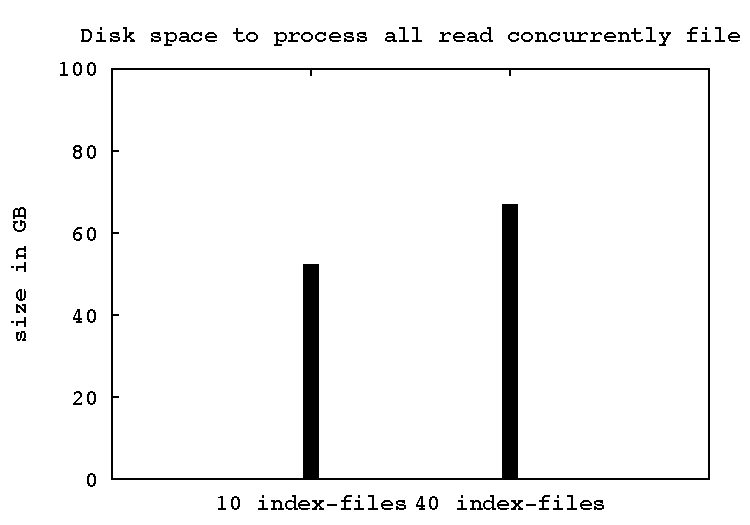
\includegraphics[scale=0.66]{figures/diskspace.pdf}
\caption{\small Disk space requirement for the cases that all read
  files are processed concurrently in a single storage (A and B). % is
%   compared to one for the cases when each single read file is
%   processed alone (C and D). 
%   Also, the cases with the low memory
%   option producing 40 index files (A and C) are compared to the cases
%   without the low memory option that produce 10 index files (B and
%   D).
}
  \label{fig:diskspace} 
 \end{figure}


\section{Mapping using Distributed, Scalable Architectures}

\subsection{Existing Solutions: Limitations and Challenges}

\jhanote{Here we need to define what solutions are currently employed,
  what works well what doesn't}

Recently, cloud computing and environments for genome-wide analysis
and infrastructure development have drawn significant attention and
interesting outcomes were reported\cite{taylor2010,cloudburst,
  cloudblast, langmead2009, langmead2010,gatk, halligan2009}

\begin{itemize*}
\item GATK\cite{gatk}
\item CloudBurst\cite{cloudburst}
\item CouldBlast\cite{cloudblast}
\item SNP finding and RNA-seq with Cloud\cite{langmead2009, langmead2010}
\end{itemize*}

In spite of successful progress from such efforts, the primary
challenges that we want to resolve, and improve are as follow.
%\begin{enumerate}
\begin{itemize*}
\item Agility for heterogeneous computing architecture
\item Extensibility and quick development cycles for a new bioinformatics tool
\item Scalability with a non-intrusive execution of a target tool  
%\end{enumerate}
\end{itemize*}


\subsection{Understanding BFAST on a Local (Single) Resource}

\subsubsection{$T_{C}$ on $N_t$ and $N_c$}

 \begin{figure}
 \centering
%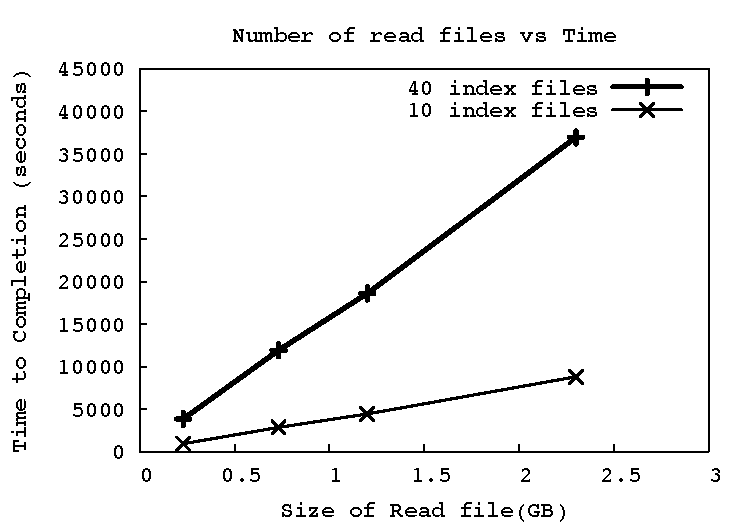
\includegraphics[scale=0.66]{figures/readsvstime.pdf}
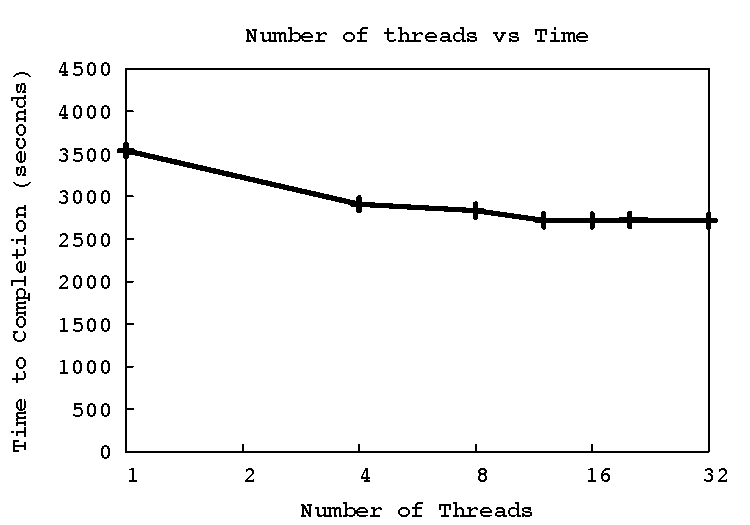
\includegraphics[scale=0.66]{figures/threadsvstime.pdf} 

\caption{\small The multi-threading capability measurement.  The
  'bfast match' 'step is measured by varying the number of cores for
  multi-threading execution.  The node tested has 12 cores.  Human
  genome (hg18) chromosome 21 is used as the reference
  genome. \jhanote{Increase y-axis resolution} }
  \label{fig:parallel-execution} 
 \end{figure}
 
To determine how the bfast match performance changes with the different number of threads and 
processor we vary the number of threads for bfast job on a single machine with multiple cores. 
The results in Fig.~\ref{fig:parallel-execution} show that the performance was better when the number 
of cores is equal to number of threads which was also recommended setting in the Bfast manual. 
Further, when we increase number of threads more than available performance does not change much. 
When less number of threads are used than the available cores the performance 
decreases but marginal around half of the cores and significant with just single thread.


So even with multi-threading option provided by bfast, the performance
could be improved by using multiple cores/threads on the same node but
it gives us only marginal overall performance gain when processing all
the read files sequentially.

... \jhanote{needs merging} The results from our investigation are presented in
Fig.~\ref{fig:parallel-execution}. First, performance gains with
multi-threading are marginal showing only 30 \% speed up when reaches
the limit with all of the number of free cores being used.  Secondly,
the multiple read file option is useful as a strategy for scaling out,
i.e. with more cores operating correspondingly a smaller read file.
Thirdly, the low memory option that creates more index files require
longer calculation time as the comparison between 40 index files $(d =
1)$ vs. 10 index files ($ d = 0 $) and $n_m = 10$.


... \jhanote{needs merging} Computational requirements vary also with
how to configure parallel/multi-threading execution patterns.  Since
BFAST provides its intrinsic support for multi-threading and parallel
execution, we examined computational requirements while varying
configurations for such parallel strategies.  For example, according
to the results shown in Fig.~\ref{fig:parallel-execution}, it is
obvious that dividing a large volume of short reads data into many
independent runs is a good strategy while multi-threading support is
limited by available cores in a same node.  Also the results in
Fig.~\ref{fig:parallel-execution} find that the low memory option that




\subsubsection{Understanding I/O}
{
To understand the how I/O of the system influences the performance of bfast matching four different experiments were conducted keeping the amount of data processed constant and number of threads  used also as constant but for the first three. In the first experiment we just perform one bfast match for  a large read file of size with four threads and four cores. In the second experiment two   bfast matches concurrently with almost half the size of read file but half of the threads   used in the first one. Similarly, in the third experiment we run four bfast matches   concurrently with almost quarter the size read file used but the in the first experiment and one thread each. Fourth one is similar to third except in the number of  threads 4 threads per bfast job is used but using just 4 cores.

 \begin{table}
 \begin{tabular}{|c|c|c|c|} 
 \hline 
Read File  & Threads per & Num. BFAST  & Time to \\
Size & BFAST taks & Tasks &  Completion \\  \hline
2.3 GB &  4 & 1 & 36942 s \\
1.2 GB & 2 & 2 & 19618 s \\
0.732 GB & 1 & 4 & 28299 s\\ 
0.732  GB & 4 & 4 & 25215 s\\

 \hline
 \end{tabular}
 \label{table:understandio} 
 \caption{Computing time for the 'bfast match' step with a single node
   (painter). Under the restriction such that the tested node has 4
   cores, the time-to-completion is compared with varying conditions
   regarding the size of read files, the number of thread for each
   'bfast match', and number of the 'bfast match' executed
   concurrently.}
\end{table}

The experiment results in Table~\ref{table:understandio} show that use of 2 threads per bfast matches simultaneously 
on a four core node is the optimal configuration for time to completion. Because it balances each thread per core but  
running the two bfast jobs per node at the same time. Thus shows advantage of running multiple bfast matches simultaneously. 


}

\jhanote{Lines 44-47 of the Excel Sheet here}

\subsection{Distributed Adaptive Runtime Environment}

To execute a scientific application using heterogeneous distributed
computing resources, we develop the Distributed Adaptive Runtime
Environment (DARE) framework\cite{dareurl}.  The framework is compose
of an open source Web application framework, Pylons and middleware of
the application management system built upon SAGA an BigJob
abstraction\cite{saga-ccgrid10,saga-royalsoc,saga-web,jha2009developing,ecmls10}.
This combination of the open source technology and the application
management system enables us to develop a lightweight, extensible,
full-fledged distributed computing science gateway quickly and
effectively\cite{pylonsurl}.

Considering a daunting size of data, in particular large genomes such as human as summarized in 
Table~\ref{table:two-genomes} and corresponding long computing times when carried out with a 
single or moderate size of clusters, parallel/concurrent execution of the target analysis with BFAST are desirable. 
 First, biological information could be utilized for such parallel execution. 
 For example, the short read sequences in fastq format could be split into many files that are 
 needed separately for parallel mapping.  At the last stage, all mapped results could be combined 
 with available tools such as SAMTools\cite{samtools}.   Additionally, a reference genome could be 
 divided into many if each dataset contains independent contigs.  For example, each chromosomes 
 or plasmids in microbes could be a separated sub-genome sequence contig.  However, note that 
 indexes of an entire contig should be used together, regardless of the low memory option that allows 
 to store indexes in many files, which is in fact the major obstacle to require a large disk space.

We implement the above data fragmentation scheme on grids and clouds with the same runtime environment using 
SAGA-BigJob\cite{saga-royalsoc,saga-ccgrid10, ecmls10}.  In our implementation, all the parallel tasks of BFAST 
steps are defined as SubJobs in BigJobs.  It is possible to assign many cores for each SubJob 
with the configuration of BigJob before submitting BigJobs. 
  
...\jhanote{needs merging} Most importantly, while the implementation
of multiple parallel tasks indicates advantages of distributed
multiple resource utilization, the large volume and variation of data
sizes associated with genome sequence data as well as minimally
required disk space needs to pay attention since in some cases, data
size itself prohibits to carry out the analysis in a computing
resource that lacks the demanded requirements, indicating the
significance of agile runtime environment that drives a dynamical
configuration and utilization of distributed resources.

\subsection{Execution on Grids and Clouds}

\subsubsection{Using BFAST On Distributed HPC Resources}

Following is the implementation described above, the execution of
mapping calculations using BFAST was tested with our runtime
environment built with the DARE framework.  Results were obtained with
a HPC grid and a Cloud environment, which demonstrate the capability
of our runtime environment for the mapping tool on distributed
heterogeneous computing resources. \jhanote{Before we say what we are
  presenting, please present a ``why and how'', i.e., outline the
  experiments}

First of all, in Table~\ref{table:bigjob-loni}, we presented the
measured time-to-completion for the step 'bfast match' with different
configurations that include the variation of the number of threading
used for each task and the number of cores (and also the number of
nodes).  These results clearly show i) effective job submission and
sub task management trough BigJob in spite of a large number of
subtasks up to 40 ii) requirement of sufficient number of cores
through available distributed computing resources (see I and II
compared to III and IV that requires many rounds of parallel
executions due to limited number of cores) that completes parallelism
with multiple read files.  In particularly, the observation with (ii),
along with the observation already shown in
Fig.~\ref{fig:parallel-execution} that observed a marginal performance
gain with the option for increasing number of threading, is clearly
supported by the results shown in Fig.~\ref{} once again that shows
the result in that without sufficient cores available from distributed
resources and dynamically adapted task distribution, achieving the
efficient execution of a target calculation is challenging.



 \begin{table}


 \begin{tabular}{|ccccc|c |} 
 \hline 
ID & BigJob Size  &  Tasks & Size of    &  Computing  \\
   & Cores(Nodes) &  & Read file &  Time\\\hline
I   & 80(8) &  40 & 0.209 GB &  1h 6m 6s \\
II  & 40(8)  &  20 & 0.435 GB & 2h 13m 51s\\
III & 12(4)  & 40  & 0.209 GB &  7h 10m 7s \\
IV & 12(4)  & 20 & 0.435 GB & 6h 37m 52s  \\
\hline
\end{tabular}
\caption{Performance comparison among parallel implementation using
  SAGA-BigJob with a HPC grid, LONI. One BigJob is submitted with the
  number of SubJobs indicated in the column for the number of tasks
  which is equivalent to the number of read files. We use two threads
  per each 'bfast   match' job.}
  \label{table:bigjob-loni} 
\end{table}


\subsubsection{Using BFAST on Clouds and Grids}

... \jhanote{needs merging} In the Grid implementation first all the
data required in the steps was transferred to machine's work directory
where we want to start the BigJob. The BFAST was installed in the home
directory and the executables path for job description of subjobs was
given accordingly.

... \jhanote{needs merging} In the cloud implementation all the data
required was transferred into the walrus because of the data size
limitation of the storage space in the running VM. Multiple VM's can
be started at once and the data in the walrus is mounted onto all the
running VM while booting the Virtual Machine. Thus all the VM can have
access to data and can process concurrently


To determine whether to use large number of small VM's or to use few
big VM's. with help of bigjob cloud implementation we designed two
experiments. In the first experiment four VM's with 2 cores each were
started and four bfast matches with one bfast on each one using SAGA
bigjob . In the second experiment a large VM with 8 cores is started
and 4 bfast jobs were launched on the same VM simultaneously using
SAGA bigjob.

 \begin{table}
 \begin{tabular}{|c|c|c|} 
 \hline 
VM's & VM type and Cores  & Time to  \\ 
&per VM& completion\\ 
\hline
4 &  2 & 1080 s \\
1 & 8 & 1020 s \\
 \hline 
 \end{tabular}
 \label{table:cloud-VM} 
 \caption{The time-to-completion is compared between the case of multiple VMs and the case of single VM}
\end{table}

Thus when same workload is distributed across multiple VM's has a
marginal gain over the one single large VM.

\jhanote{Need to refer to Table\ref{table:cloud-VM}}


\section{Concluding Remarks}
We present our analyses with two genome systems representing a
eukaryote and a prokaryote, respectively, using a HPC grid and a Cloud
environment for an understanding of conditions of a scalable
cyberinfrastructure for an effective execution of mapping, and
consequently genome-wide analyses.  Based on our results, we conclude
that an infrastructure to run with a proper configuration for
concurrent tasks benefits genome-wide analysis and such a
configuration is optimized only when parameters from biological
contexts as well as limitations and potentials of distributed
computational resources are taken into account together.  For that
purpose, our DARE framework provides an efficient solution.



\bibliographystyle{abbrv}
\bibliography{ecmls11}


\end{document}


% in addition to the requirement of an uderstanding of applications of
% interest in terms of the capability of parallel execution in
% heterogeneous computing environment,

% and importantly, difficulties of utilization of heterogeneous
% distributed computing resources

% This is partly because, in addition to requirement of an understanding
% of applications of interest in terms of the capability of parallel
% execution in heterogeneous computing environment, the complexity of
% biological contexts associated with characteristics of a target
% genome(s), the volume of relevant genomics data, and importantly,
% difficulties of utilization of heterogeneous distributed computing
% resources constitute challenges for introducing an appropriate
% scalable architecture for the infrastructure.

% required software is relatively less
% recognized for its significance.  

% The need of computational methods as well as computing architectures
% for compute-intensive and data-intensive calculations for resolving
% new challenges arising from requirements of processing and analyzing
% genome sequencing data, therefore, is regarded indispensable for
% accurate and reliable analysis against high-throughput sequencing data
% and following genome-wide analyses.

%% As a result, remarkable advances have been witnessed in recent years
%% and a number of bioinformatics tools aiming to solve emerging
%% challenges are currently available to the scientific
%% community\cite{trapnell2009,bfast2009,scheibye-alsing2009,pepke2009,samtools}.

% The need of such infrastructures is also understood with
% catastrophically growing datasets for genomics and their applications
% for public heath issues.

% Nonetheless, some interesting progresses are recently reported, for
% example, with the utilization of emerging computing architecture such
% as Cloud\cite{taylor2010}

% \jhanote{we want to present a strawman of an architecture based upon
%   requirements and a reference implementation of the architecture}
